\section{Multigrid Laplacian Implementation}

In this section a one-dimensional solution to Laplace's equation is described using CAFe
syntax.  The solution uses multigrid techniques to improve the rate of convergence
of iterative methods.  We describe the implementation in terms of a one-dimensional
problem for simplicity.

\subsection{Multigrid Algorithm}

The multigrid algorithm uses a series of successively coarser grids to
iteratively approximate the solution obtained from the preceding
finer grid.  Higher frequency error modes are damped out as the
solution processes up the grid hierarchy.  At the top of the
hierarchy, an exact solution is obtained and then this solution is
iterated and propagated down the grid hierarchy form coarser to finer
grids.  After a few sweeps up and down the hierarchy the solution will
have been obtained on the desired original grid.

\begin{figure}[!t]
\centering
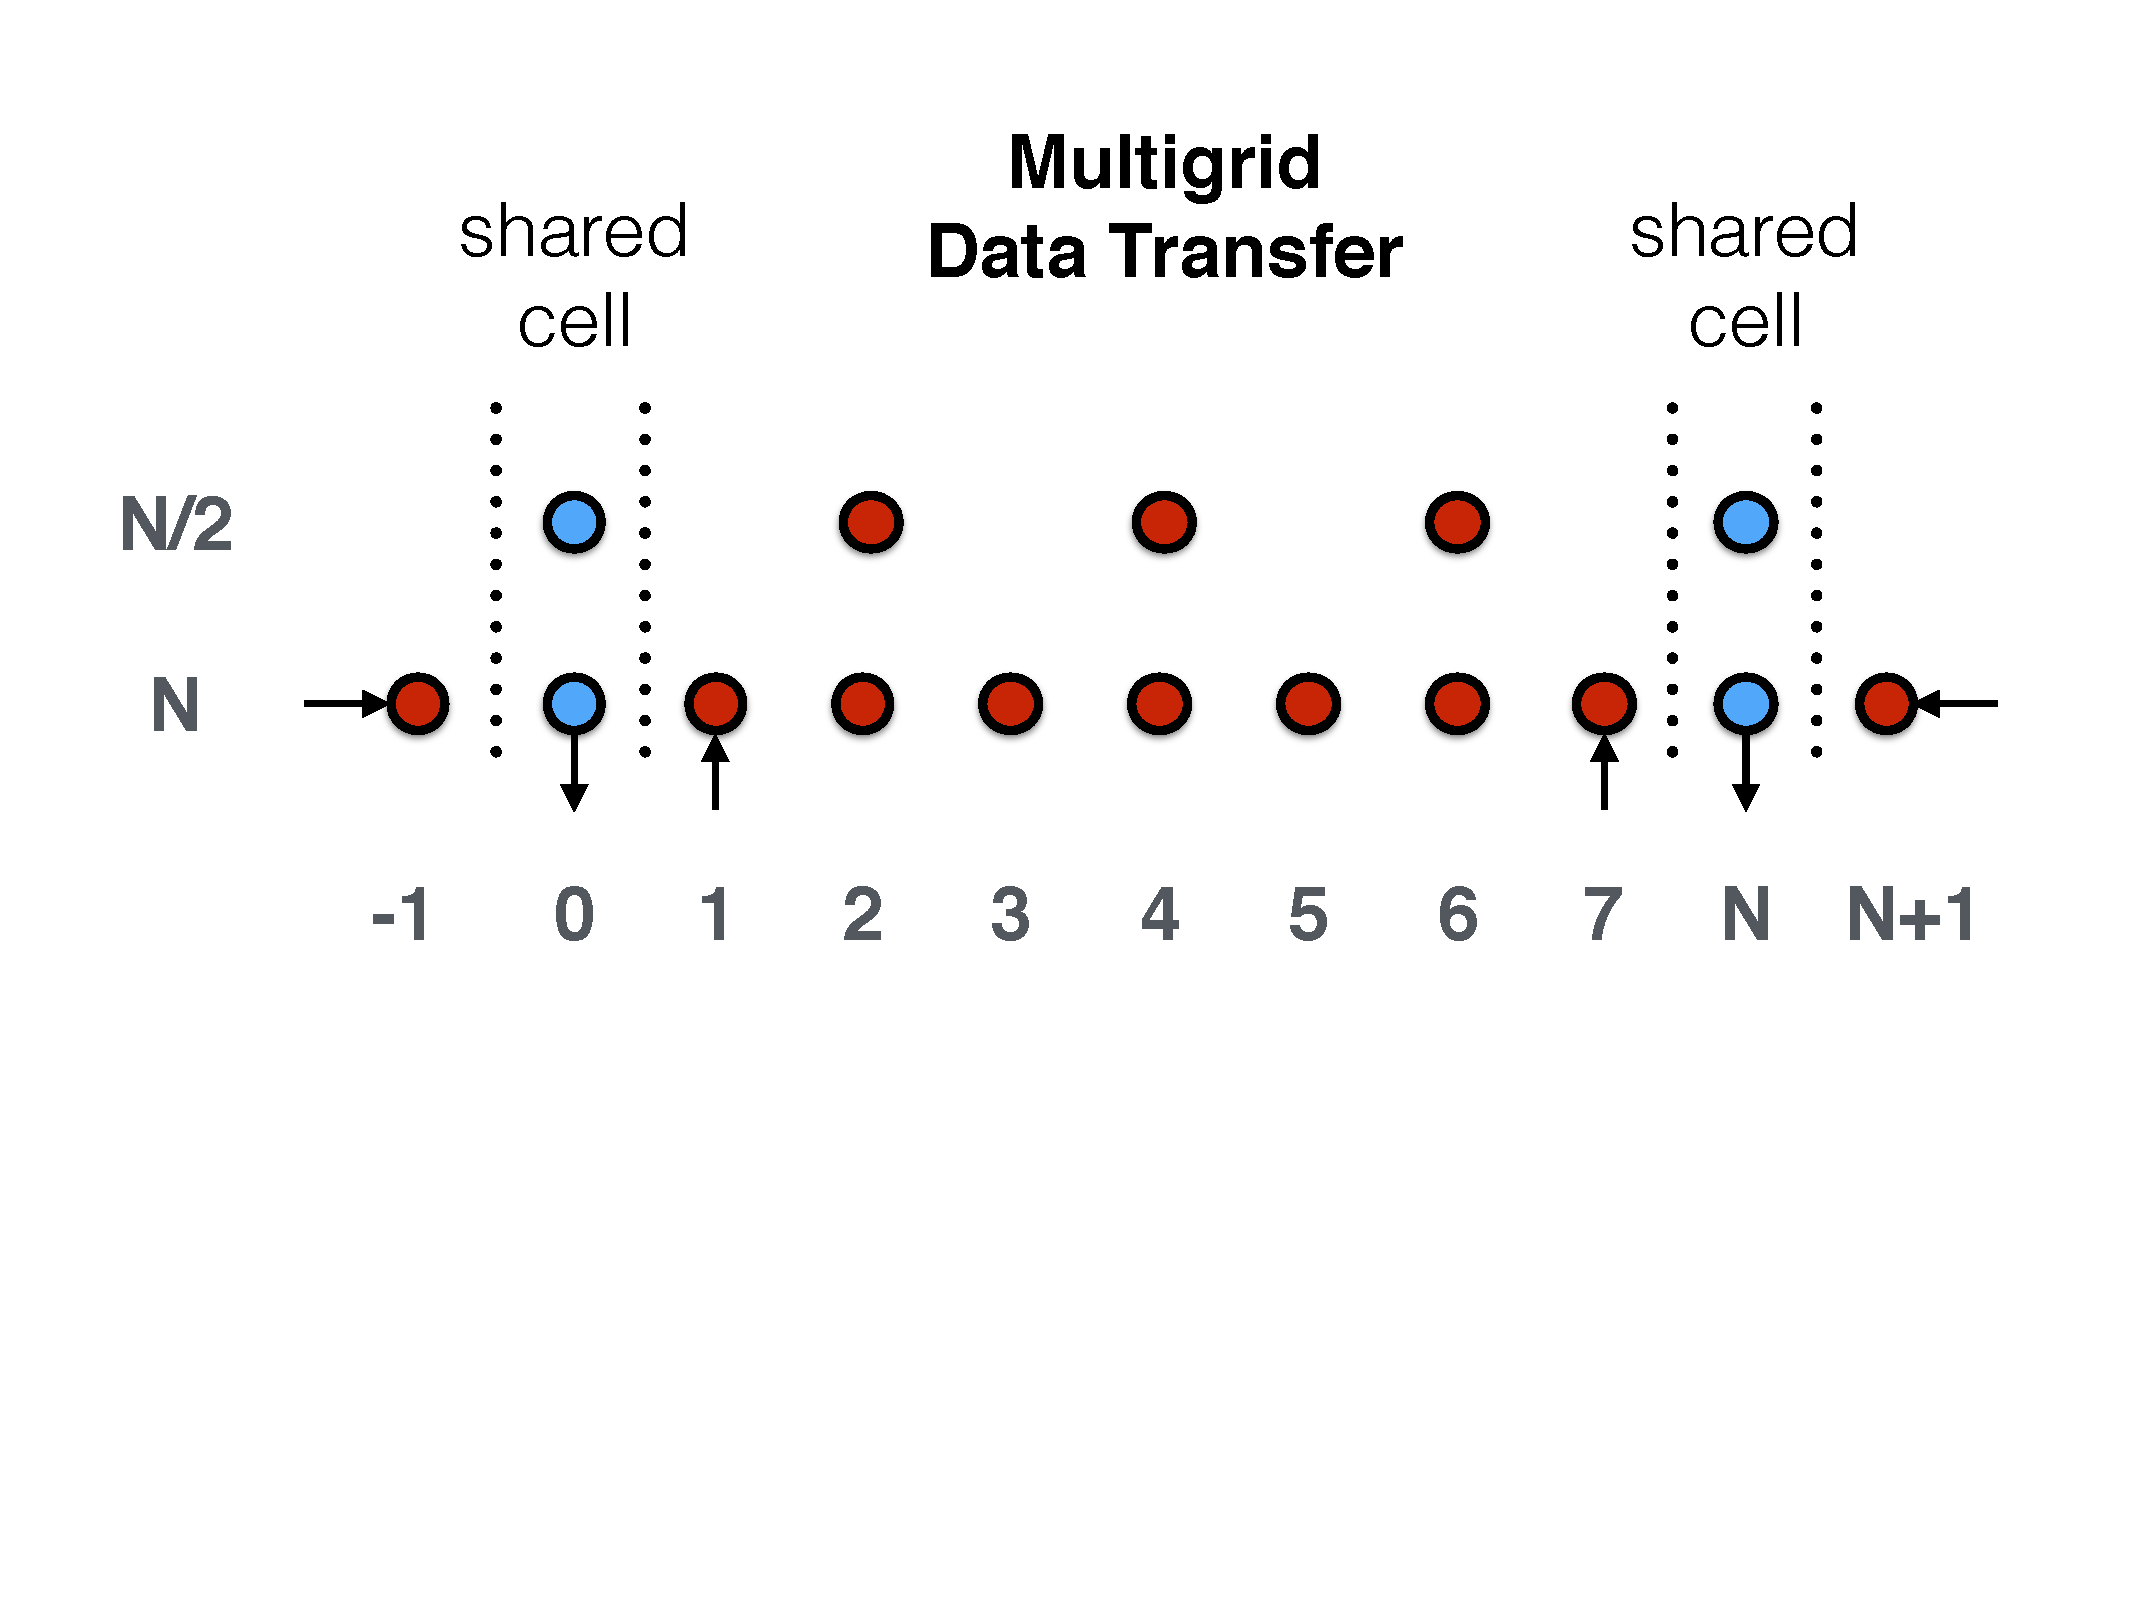
\includegraphics[width=2.5in]{Fig1}
\caption{Two multigrid levels (N,N/2) on one image showing the two cells that are shared with
  neighbors on the left and the right and computed redundantly.  The fine level grid (N)
  also shows the two cells that must be exchanged between neighbors.  Arrows represent the direction
  of data exchange from the perspective of the local image.}
\label{fig_grids}
\end{figure}

Two levels of the grid hierarchy are shown in Fig. \ref{fig_grids} running on a processor computing on
an interior portion of the grid; additional images are computing on regions to the left and right of
the region shown in the figure.  The finest grid (size N) is shown
in the bottom of the figure with cell indices running from (-1:N+1).  Cells 0 and N are shared
between image neighbors to the left and right (indicated by the light blue coloring and the vertical
dashed lines).  These shared cells are computed redundantly on each program image.

The red cells in the figure are computed concurrently on all subimages (one per image).
This distribution of computation over the hierarchical domain of images and subimages
requires communication of boundary regions between the various computational resources.
The communication is shown by arrows in the grid level N of the figure.  Data in cells 1
and 7 must be transferred from the subimage (upwardly pointing arrows) and the shared cell
computations must be copied to the subimage (downwardly pointing arrows). The horizontal
arrows represent data computed and subsequently transferred from the left and right
neighbors.

\begin{figure}[!t]
\centering
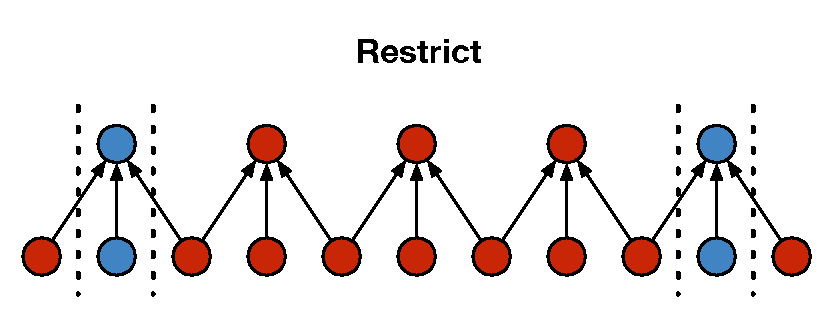
\includegraphics[width=2.5in]{Fig2}
\caption{Restriction of fine grid to coarse grid. Arrows show the points used in
         mapping onto the coarse grid.}
\label{fig_restric}
\end{figure}

The second grid level N/2 is also shown in Figure \ref{fig_grids}.  Data on this grid is obtained
by simple interpolation from information on grid level N as shown in Figure \ref{fig_restric}.
We call this interpolation a restriction and refer the reader to previous work on the multigrid
technique for more information\cite{multigrid_methods}.  The approximate solution on the N/2
grid is relaxed a few times and then passed on to grid level N/4 for further iteration.

\begin{figure}[!t]
\centering
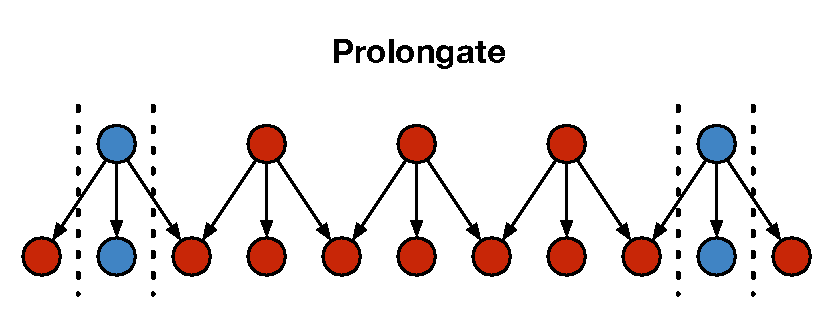
\includegraphics[width=2.5in]{Fig3}
\caption{Prolongation of coarse grid to fine grid. Arrows show the points used to
         interpolate onto the fine grid.}
\label{fig_prolongate}
\end{figure}

At the top of the grid hierarchy there are sufficiently few cells that an exact solution can be
obtained (perhaps by a non-iterative method).  This solution is then propagated down the
grid hierarchy as shown in Figure \ref{fig_prolongate}.

\subsection{Implementation of the Relaxation Step}

The multigrid algorithm has been implemented in Fortran using the CAFe
syntax described in the previous section. Data coarrays at each grid
level are declared, allocated, and initialized on each program image.
These coarrays are then copied to the subimages by the parent, hosting
images.  Below we show the implementation of the relaxation loop on
grid level N.  Each iteration step incorporates concurrent computation
on an image and its hosted subimage.  In order to execute
concurrently, we must declare an event variable to allow concurrent
execution and then synchronization once computation on \emph{both} 
the subimage \emph{and} the image have completed.

The event variable is declared as,
%%\small
\begin{verbatim}
 type(event_type) :: evt
\end{verbatim}
%%\normalsize
After initialization, this event variable has its count variable set to 0 and is incremented
each time the subimage task completes during an iteration of the code segment shown below:

\vskip 20pt

\small
\begin{verbatim}
 do i = 1, nsteps                            1
   call relax (N, V1h[dev], Buf[dev])        &
                    [[dev, EVENT=evt]]       2
   call relax_boundary (N, V1h)              3

   wait event (evt, until_count=i)           4

   V1h(0)[dev] = V1h(0)                      5
   V1h(N)[dev] = V1h(N)                      6

   V1h(  1) = V1h(  1) [dev]                 7
   V1h(N-1) = V1h(N-1) [dev]                 8

   sync all                                  9

   V1h( -1) = V1h(N-1) [left]               10
   V1h(N+1) = V1h(  1) [right]              11

   sync all                                 12
 end do                                     13
\end{verbatim}
\normalsize

This example shows the first relaxation steps on the finest grid level N.  The initial
guess (provided by the coarray \texttt{V1h}) is relaxed \texttt{nsteps} times as
specified by the loop beginning at statement 1.  The relaxation is computed on
the subimage \texttt{dev} by the call to the \texttt{relax} procedure at statement 2.
This call uses coarray memory located on the subimage as specified by the arguments
\texttt{V1h[dev]} and \texttt{Buf[dev]}, where the second coarray is used for temporary
storage.

Since an event \texttt{evt} has been supplied to the call in statement 2, the program
continues execution without waiting for the remote task on \texttt{dev} to complete.  The
count associated with the event will be increased by an implicit post to the event once
the task has finished executing.  Thus the task started by statement 2 will execute
concurrently with the \texttt{relax\_boundary} call at statement 3 --- the first call
executes on the subimage \texttt{dev} while the second call executes on the local image
\texttt{this\_image()}.

Most of the computation is accomplished by the subimage executing the \texttt{relax}
procedure (not shown) operating over the interior corresponding to fine grid indices (1:N-1).
Concurrently, \texttt{relax\_boundary} operates on the boundary indices 0 and N
(note that memory for the boundary computation is located on local image as
the coarray \texttt{V1h} is not coindexed using square bracket notation in statement 3.

Once relaxation of the boundary has completed, the program image will wait for the event
indicating that the subimage task has finished executing relaxation on the interior (statement
4).  The \texttt{until\_count} for the event is increased by 1 each iteration of the loop,
so the program waits until the event counter equals the iterate counter \texttt{i}.

Once the wait has completed, communication of the halo regions between the subimage and
the hosting image can begin.  Shared boundary cells at 0 and N are copied \emph{to} the
subimage by the execution of statements 5 and 6 and interior regions at cells 1 and N-1 are
copied \emph{from} the subimage by statements 7 and 8.  Boundary cells are exchanged (copied)
from neighboring images by statements 10 and 11.  To ensure that no race conditions are
introduced by the exchange of information between images, explicit synchronization is
accomplished by the execution of statements 9 and 12.

\begin{comment}
There are four points to note regarding this memory allocation: 1. Memory is only allocated if a
subimage has been obtained; 2. The location where memory is allocated is denoted by regular coarray
notation \texttt{U[device]}; 3. The allocated size and halo attribute of the new array are obtained
from the previously allocated local array \texttt{U} via the notation \texttt{HALO\_SRC=U} (using
\texttt{HALO\_SRC} will also initially copy \texttt{U} to the subimage); and finally 4. The
allocation itself is \emph{executed} on the subimage device with the notation \texttt{[[device]]}.

Fortran uses square bracket notation, e.g. \texttt{[image]}, to specify on what process the
memory reference is physically located.  Square brackets are a visual clue to the
programmer that the memory reference may be remote and therefore potentially suffer a
performance penalty.  CAFe extends this by employing double-bracket notation to indicate
possibly \emph{remote subimage execution}.

Note that a transfer of halo memory is necessary after each completion of the do concurrent loop.
This must be done in order for the halo region of a coarray on a given process to be consistent
with the corresponding interior of the coarray on a logically neighboring process.
Finally, memory for the entire array \texttt{U} can be copied from the
subimage device with the statement,
\texttt{U = U[device]}, 
and memory deallocation (not shown) is similar to memory allocation.
\end{comment}
